\begin{frame}
\frametitle{Non-Euclidean geometry}
\begin{columns}[c]
\column{0.7\textwidth}
\begin{itemize}
\item Distances are not always measured along a straight line.\par
\item Sometimes we want distances measured on a manifold.\par
\item Shortest path on a manifold is along a \emph{geodesic}.
\end{itemize}
\column{0.3\textwidth}

\includegraphics[width=\textwidth]{Globe}
\end{columns}
Linear trajectory\par

\includegraphics[width=\textwidth]{series1}\par
Nonlinear trajectory\par

\includegraphics[width=\textwidth]{series2}\par
\end{frame}

%\begin{frame}
%\frametitle{Metric distances}
%Fly in a straight line, but the path is curved.\par
%\begin{center}
%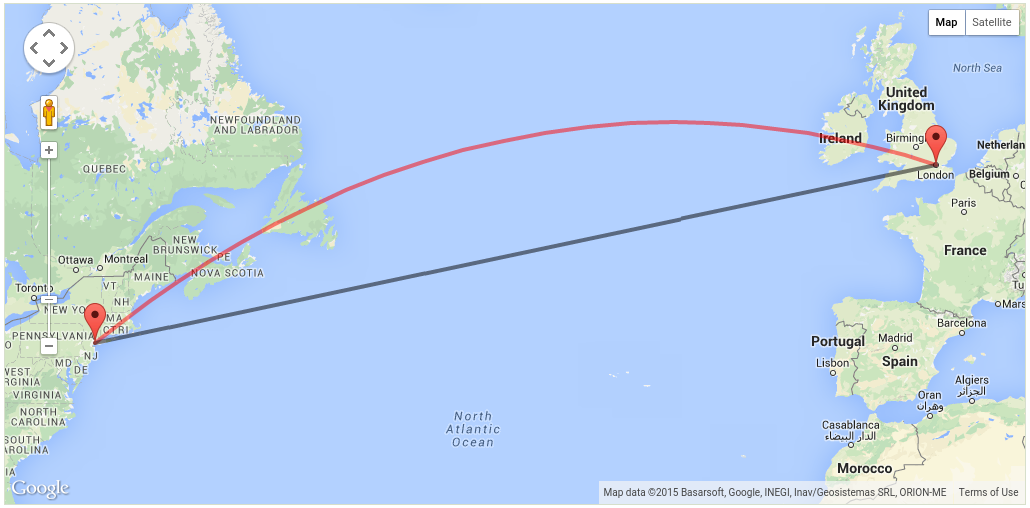
\includegraphics[width=.9\textwidth]{NewYork-London}
%\end{center}
%
\includegraphics[width=\textwidth]{series2}\par
%\end{frame}


\begin{frame}
\frametitle{Metric distances}
Distances should satisfy the properties of a \emph{metric}:
\begin{enumerate}
\item $d({\bf x}, {\bf y}) \ge 0$ (non-negativity)
\item $d({\bf x}, {\bf y}) = 0$ if and only if ${\bf x} = {\bf y}$ (identity of indiscernibles)
\item $d({\bf x}, {\bf y}) = d({\bf y}, {\bf x})$ (symmetry)
\item $d({\bf x}, {\bf z}) \le d({\bf x}, {\bf y}) + d({\bf y}, {\bf z})$ (triangle inequality).
\end{enumerate}

Satisfying (3) requires inverse-consistent image registration.

Satisfying (4) requires a specific class of image registration models.


\includegraphics[width=\textwidth]{series2}\par
\end{frame}

\begin{frame}
\frametitle{Computing a metric distance}
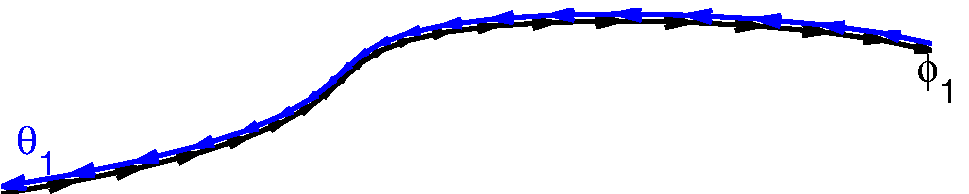
\includegraphics[width=\textwidth]{trajectory0}\par
\begin{columns}[c]
\column{0.8\textwidth}
Decompose a curved path into a series of short line segments, and add the lengths of the segments together.\par
\column{0.2\textwidth}

\includegraphics[width=\textwidth]{Globe}
\end{columns}

\includegraphics[width=\textwidth]{series2}
\end{frame}


%%%%%%%%%%%%%%%%%%%%%%%%%%%%%%%%%%%%%%%%%%%%%%%%%%%%%%%%%%%%%%%
\begin{frame}
\frametitle{Computing large deformations}
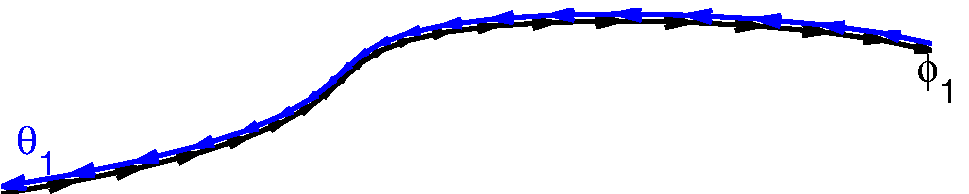
\includegraphics[width=\textwidth]{trajectory0}\par
We can consider a large deformation as the composition of a series of small deformations:
\begin{eqnarray*}
{\boldsymbol\varphi}_{1} = \left(\mathrm{Id} + {\bf v}_{t_{N-1}}\right) \circ  \left(\mathrm{Id} + {\bf v}_{t_{N-2}}\right) \circ ... \circ \left(\mathrm{Id} + {\bf v}_{t_1}\right) \circ \left(\mathrm{Id} + {\bf v}_0\right)
\end{eqnarray*}

The inverse of the deformation can be computed from:
\begin{eqnarray*}
{\boldsymbol\vartheta}_{1} = \left(\mathrm{Id} - {\bf v}_0\right) \circ  \left(\mathrm{Id} - {\bf v}_{t_1}\right) \circ ... \circ \left(\mathrm{Id} - {\bf v}_{t_{N-2}}\right) \circ \left(\mathrm{Id} - {\bf v}_{t_{N-1}}\right)
\end{eqnarray*}

\end{frame}

%%%%%%%%%%%%%%%%%%%%%%%%%%%%%%%%%%%%%%%%%%%%%%%%%%%%%%%%%%%%%%%

\begin{frame}
\frametitle{Metric distances from large deformations}
By modelling trajectories as piecewise linear, distances can be computed by adding the distances from the small deformations:
\begin{eqnarray*}
d = \frac{1}{N}\sum_{n=0}^{N-1} || {\bf L} {\bf v}_{t_n} ||
\end{eqnarray*}
%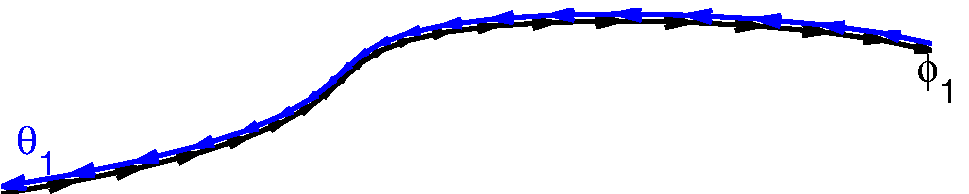
\includegraphics[width=\textwidth]{trajectory0}

If $N$ approaches infinity (and we use small deformations of $Id + \frac{1}{N}{\bf v}_t$), the evolution of a deformation may be conceptualised as integrating the following equation:
\begin{eqnarray*}
\frac{d {\boldsymbol\varphi}}{d t} = {\bf v}_t ({\boldsymbol\varphi})
\end{eqnarray*}

Geodesic distances (from zero) are then measured by:
\begin{eqnarray*}
d = \int_{t=0}^1  || {\bf L} {\bf v}_t || dt
\end{eqnarray*}
\end{frame}

\begin{frame}
\frametitle{Metric distances from large deformations}
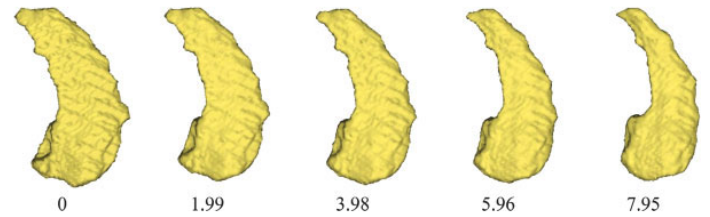
\includegraphics[width=\textwidth]{hippocampi}\par
\begin{tiny}
Miller et al. ``Collaborative computational anatomy: an MRI morphometry study of the human brain via diffeomorphic metric mapping.'' Human Brain Mapping 30(7):2132--2141 (2009).\par
\end{tiny}
\end{frame}

\begin{frame}
\frametitle{Metric distances from large deformations}
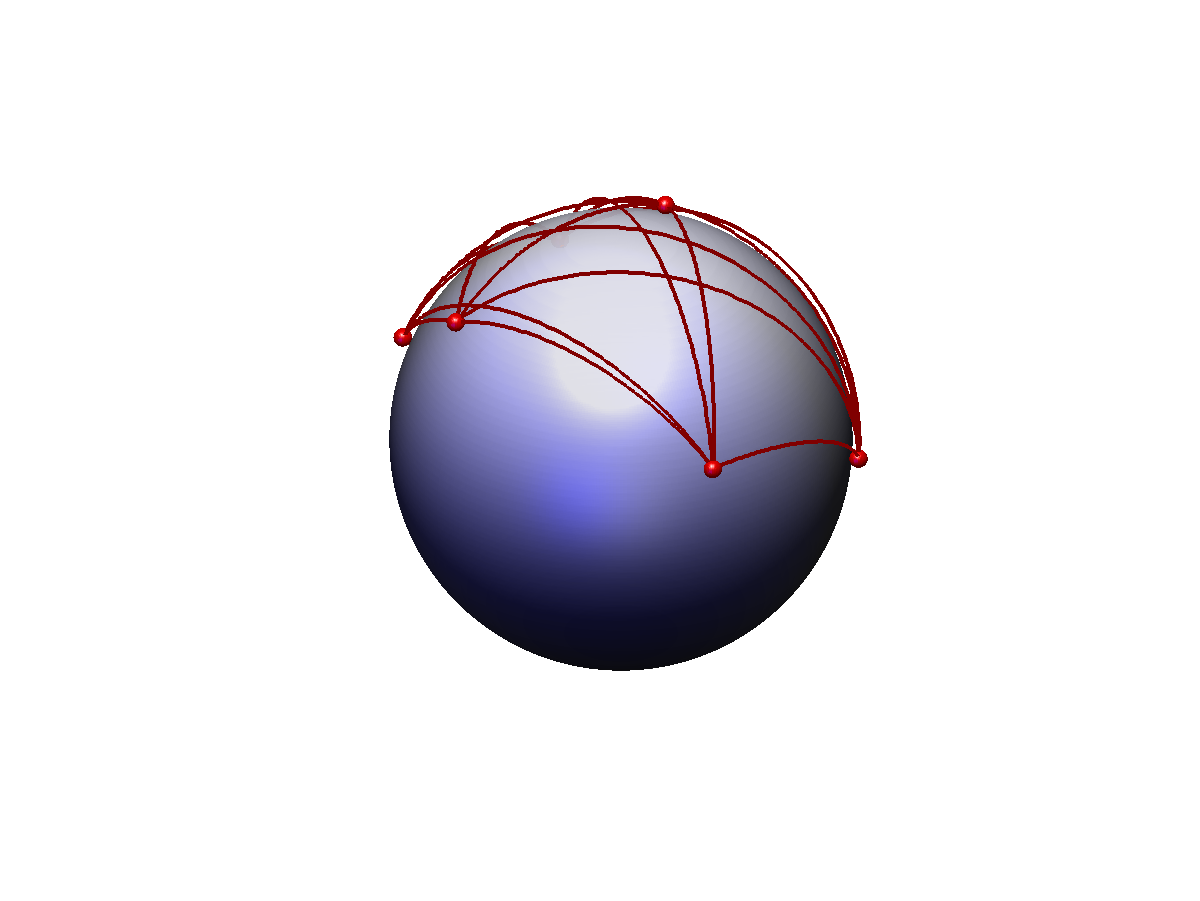
\includegraphics[width=.8\textwidth]{metric_distances}\par
\begin{tiny}
Miller et al. ``Collaborative computational anatomy: an MRI morphometry study of the human brain via diffeomorphic metric mapping.'' Human Brain Mapping 30(7):2132--2141 (2009).\par
\end{tiny}
\end{frame}

